\documentclass[aspectratio=169,11pt]{beamer}

\usetheme{Madrid}
\usecolortheme{default}
\usefonttheme{professionalfonts}
\setbeamertemplate{navigation symbols}{}
\setbeamertemplate{footline}[frame number]

\usepackage{amsmath, amssymb, booktabs, graphicx}
\graphicspath{{../../assets/figures/}{assets/figures/}}

\title{Personnel Economics and Internal Labor Markets}
\subtitle{Labor II --- Week 3}
\author{Teaching deck draft}
\date{}

\begin{document}

\begin{frame}
  \titlepage
\end{frame}

\begin{frame}{Central question and course positioning}
\begin{itemize}
    \item Once the firm has chosen employment and adjustment speed, how should it organize workers inside the firm?
    \item Week 3 stays on the firm side: incentives, promotions, teams, managers, and workplace rules.
    \item Week 4 moves outward to search, turnover, vacancies, and unemployment flows.
\end{itemize}
\end{frame}

\begin{frame}{Week 2 to Week 3 bridge}
\begin{itemize}
    \item Week 2 asked why firms do not move instantly to their labor-demand target.
    \item Week 3 asks why two firms with similar workforces can still have very different productivity, retention, and promotion outcomes.
    \item Adjustment costs tell us why employment paths are slow; personnel economics tells us how firms govern the workers they have.
\end{itemize}
\end{frame}

\begin{frame}{What personnel economics studies inside firms}
\[
Y = F\big(K, L, e(\omega), m, T\big)
\]

\begin{itemize}
    \item Internal organization changes output through effort, supervision, and team structure, not only through headcount.
    \item The key objects are incentives, evaluation, assignment, promotion, and workplace practices.
    \item This is labor economics inside firms, not a separate management detour.
\end{itemize}
\end{frame}

\begin{frame}{Course map}
\begin{center}
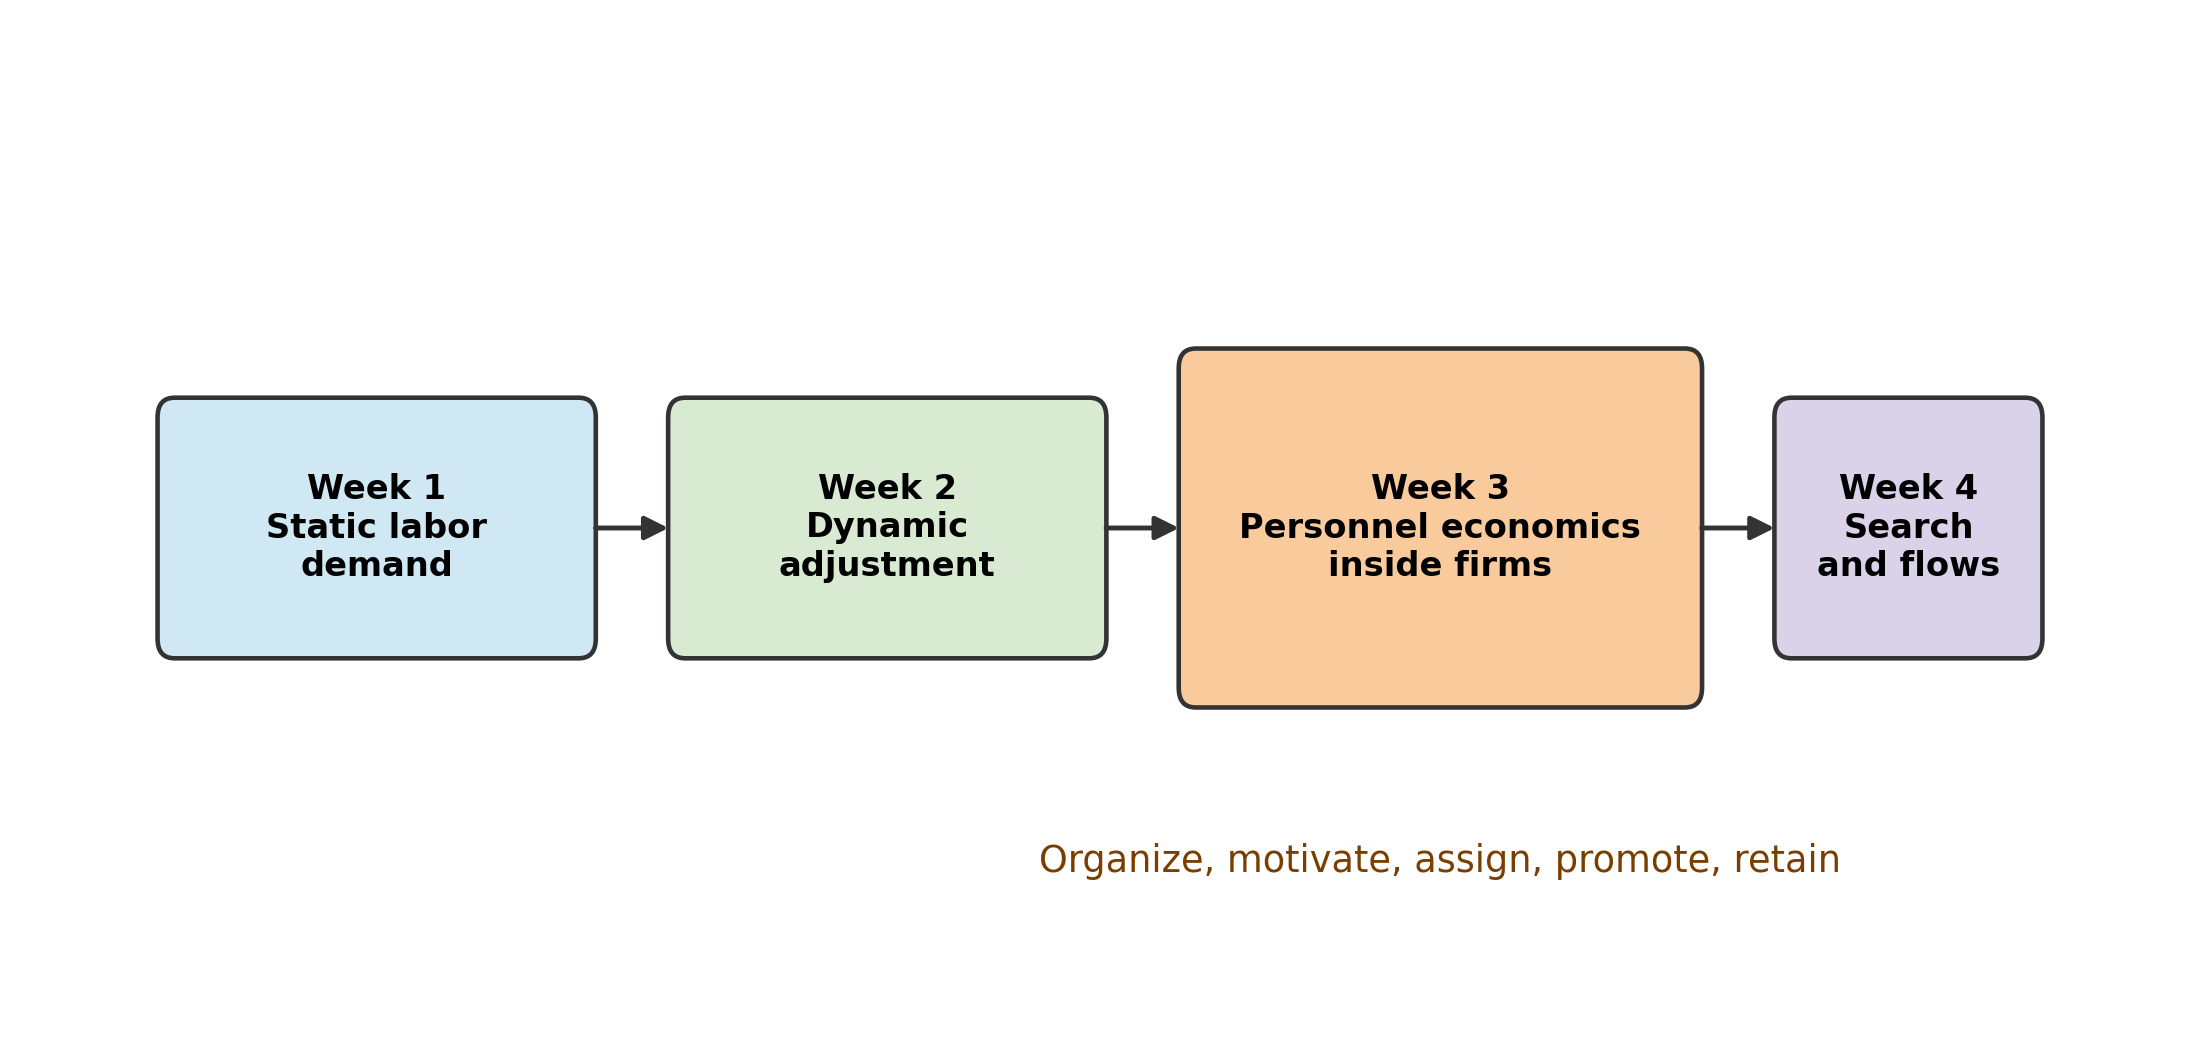
\includegraphics[width=0.88\linewidth]{03-personnel-economics-in-course-map.png}
\end{center}
\end{frame}

\begin{frame}{Incentives, compensation, and agency}
\[
e_i = e\big(w_i, b_i(y_i), p_i, \text{monitoring}_i\big)
\]

\begin{itemize}
    \item Fixed pay, bonus pay, promotions, and monitoring are joint instruments.
    \item Incentives can change effort today and selection into the job tomorrow.
    \item Firm experiments are strongest for within-firm treatment effects, weaker for transportability.
\end{itemize}
\end{frame}

\begin{frame}{Multitasking, subjective evaluation, and career incentives}
\[
q_i = \theta_1 a_{i1} + \theta_2 a_{i2} + \varepsilon_i
\]

\begin{itemize}
    \item Measured output is often an incomplete proxy for firm value.
    \item Narrow performance pay can distort task allocation.
    \item Subjective evaluation and promotions help repair missing information, but they add opacity and politics.
\end{itemize}
\end{frame}

\begin{frame}{Incentives and promotions connect current and future jobs}
\begin{center}
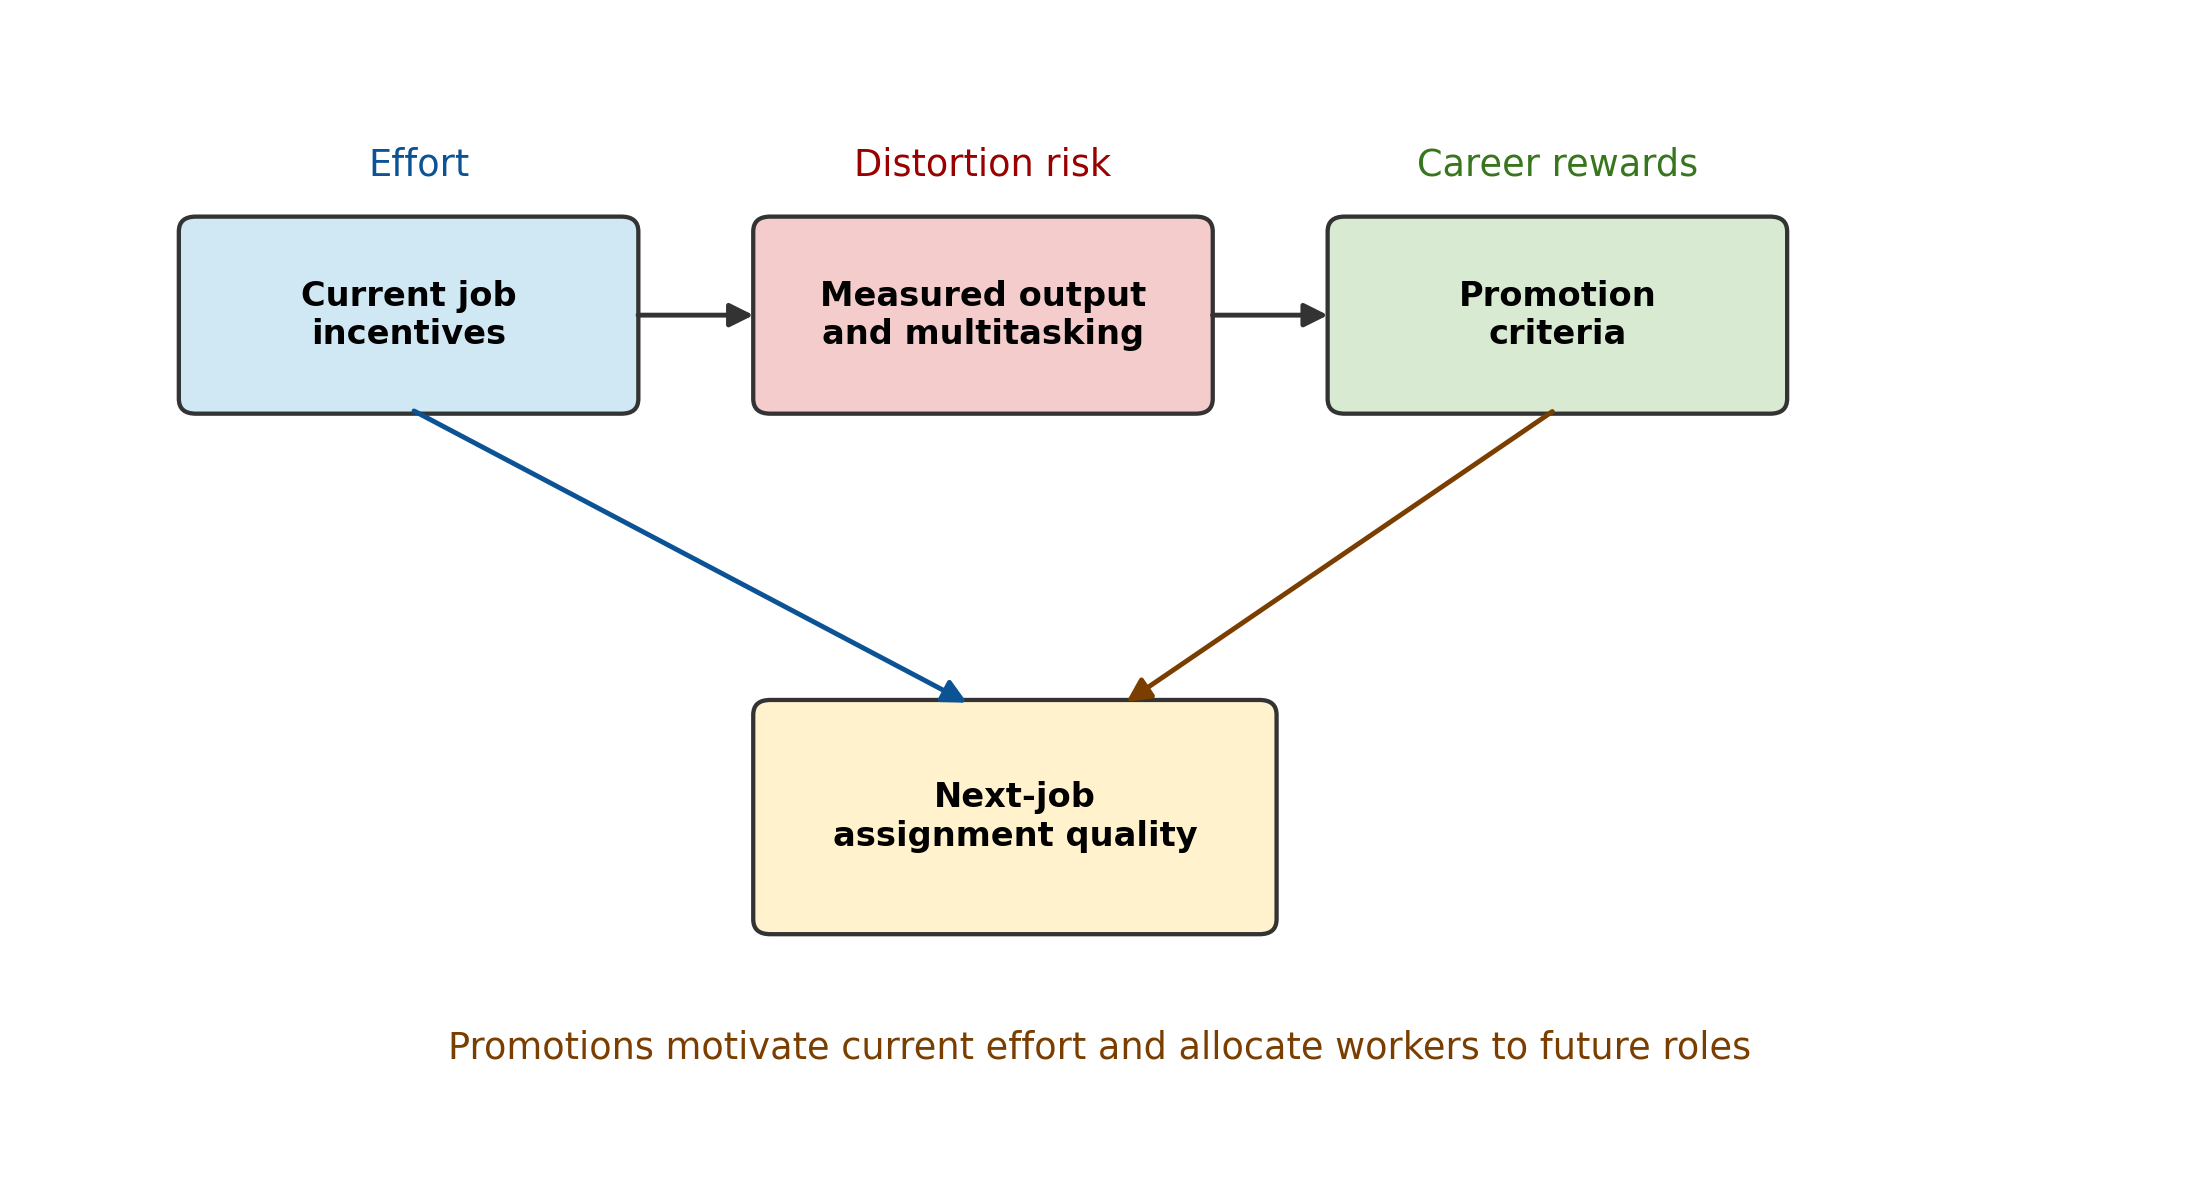
\includegraphics[height=0.68\textheight]{03-incentives-assignment-promotion.png}
\end{center}
\end{frame}

\begin{frame}{Promotions, assignment, and the Peter Principle}
\[
\Pr(\text{promote}_i=1) = g\big(y_i, z_i, \widehat{m}_i\big)
\]

\begin{itemize}
    \item Promotions are both incentives in the current job and assignments into the next job.
    \item Promoting the best current performer need not produce the best future manager.
    \item Benson, Li, and Shue turns the Peter Principle into a measurable personnel-data object.
\end{itemize}
\end{frame}

\begin{frame}{Managers, peers, and teams}
\[
y_i = a_i e_i + \rho \bar e_{-i} + u_i
\]

\begin{itemize}
    \item Manager effects, peer effects, and team complementarities are distinct channels.
    \item Team incentives can internalize complementarities but can also invite free-riding.
    \item Management-practice measurement is not the same as a causal management shock.
\end{itemize}
\end{frame}

\begin{frame}{Managers, peers, and spillovers}
\begin{center}
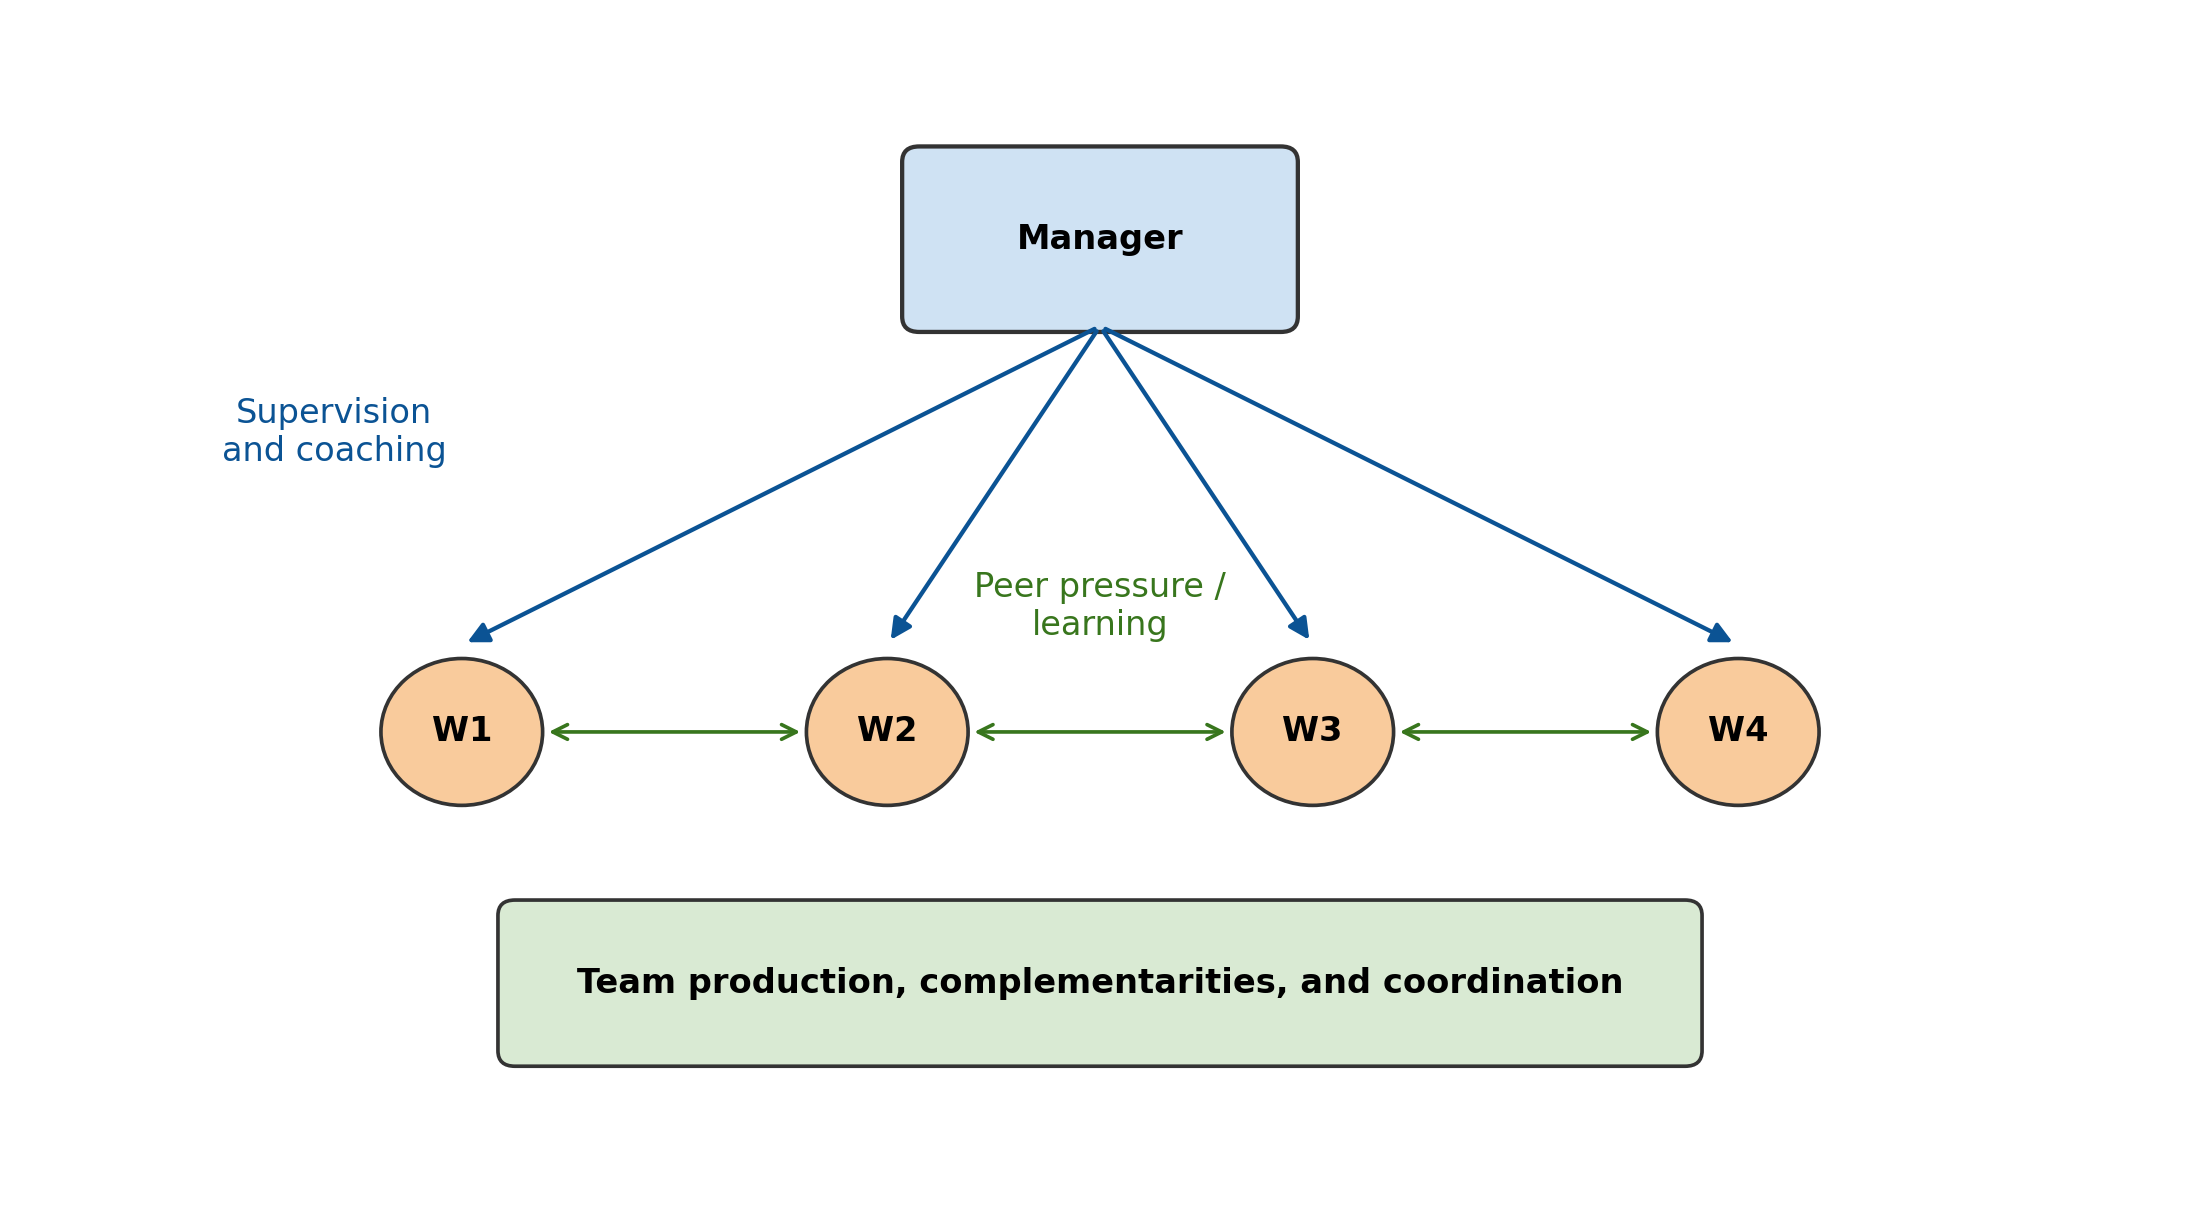
\includegraphics[height=0.68\textheight]{03-managers-peers-teams.png}
\end{center}
\end{frame}

\begin{frame}{Data, designs, and external validity}
\small
\begin{tabular}{p{0.25\linewidth} p{0.22\linewidth} p{0.18\linewidth} p{0.23\linewidth}}
\toprule
Design & Variation & Margin & Core caveat \\
\midrule
Firm experiment & Incentives or teams & Output, profit & Narrow external validity \\
Internal policy change & Rollout or criteria & Productivity, retention & Endogenous adoption \\
Personnel records & Promotions, switches & Assignment, careers & Selective reallocation \\
Management survey & Practices across firms & Productivity, wages & Measurement vs causality \\
Digital trace or policy shock & Communication, rules & Workflow, quits, inequality & Proprietary or bundled channels \\
\bottomrule
\end{tabular}
\end{frame}

\begin{frame}{Data and design map}
\begin{center}
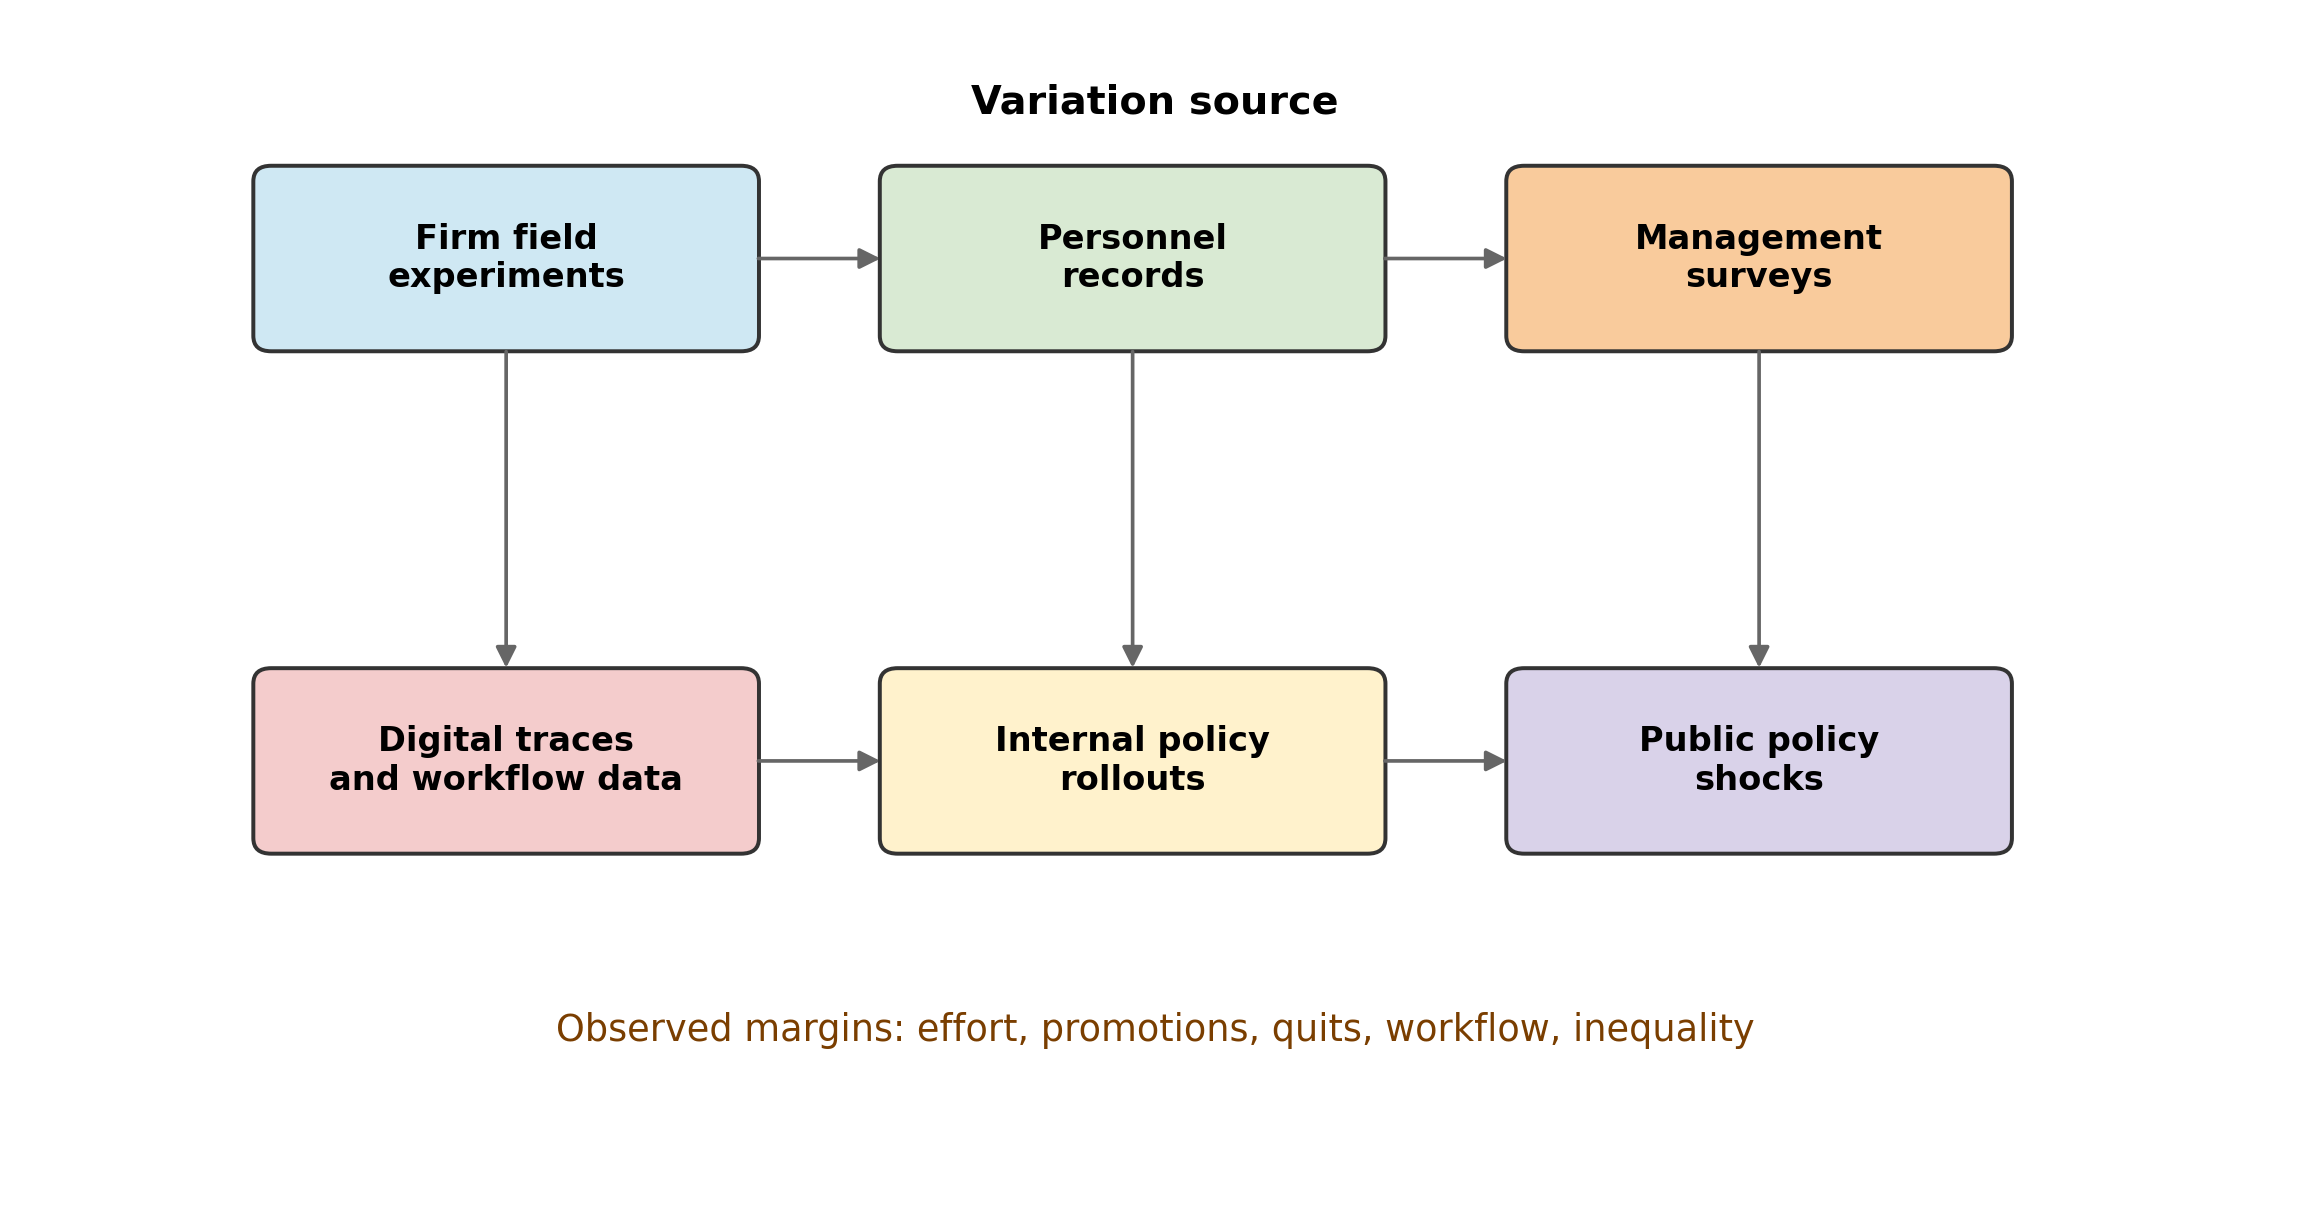
\includegraphics[height=0.68\textheight]{03-data-design-frontier-map.png}
\end{center}
\end{frame}

\begin{frame}{Frontier extension}
\begin{itemize}
    \item Managers below the C-suite: who becomes a good manager, and when is quality portable?
    \item Remote work: separate selection from treatment before interpreting productivity or promotion gaps.
    \item Voice, communication, and internal governance: policy can change workplace organization from outside the firm.
    \item Digital traces, algorithmic management, AI, and training: new data make internal organization observable but raise new interpretation risks.
\end{itemize}
\end{frame}

\begin{frame}{Research opportunities landscape}
\begin{center}
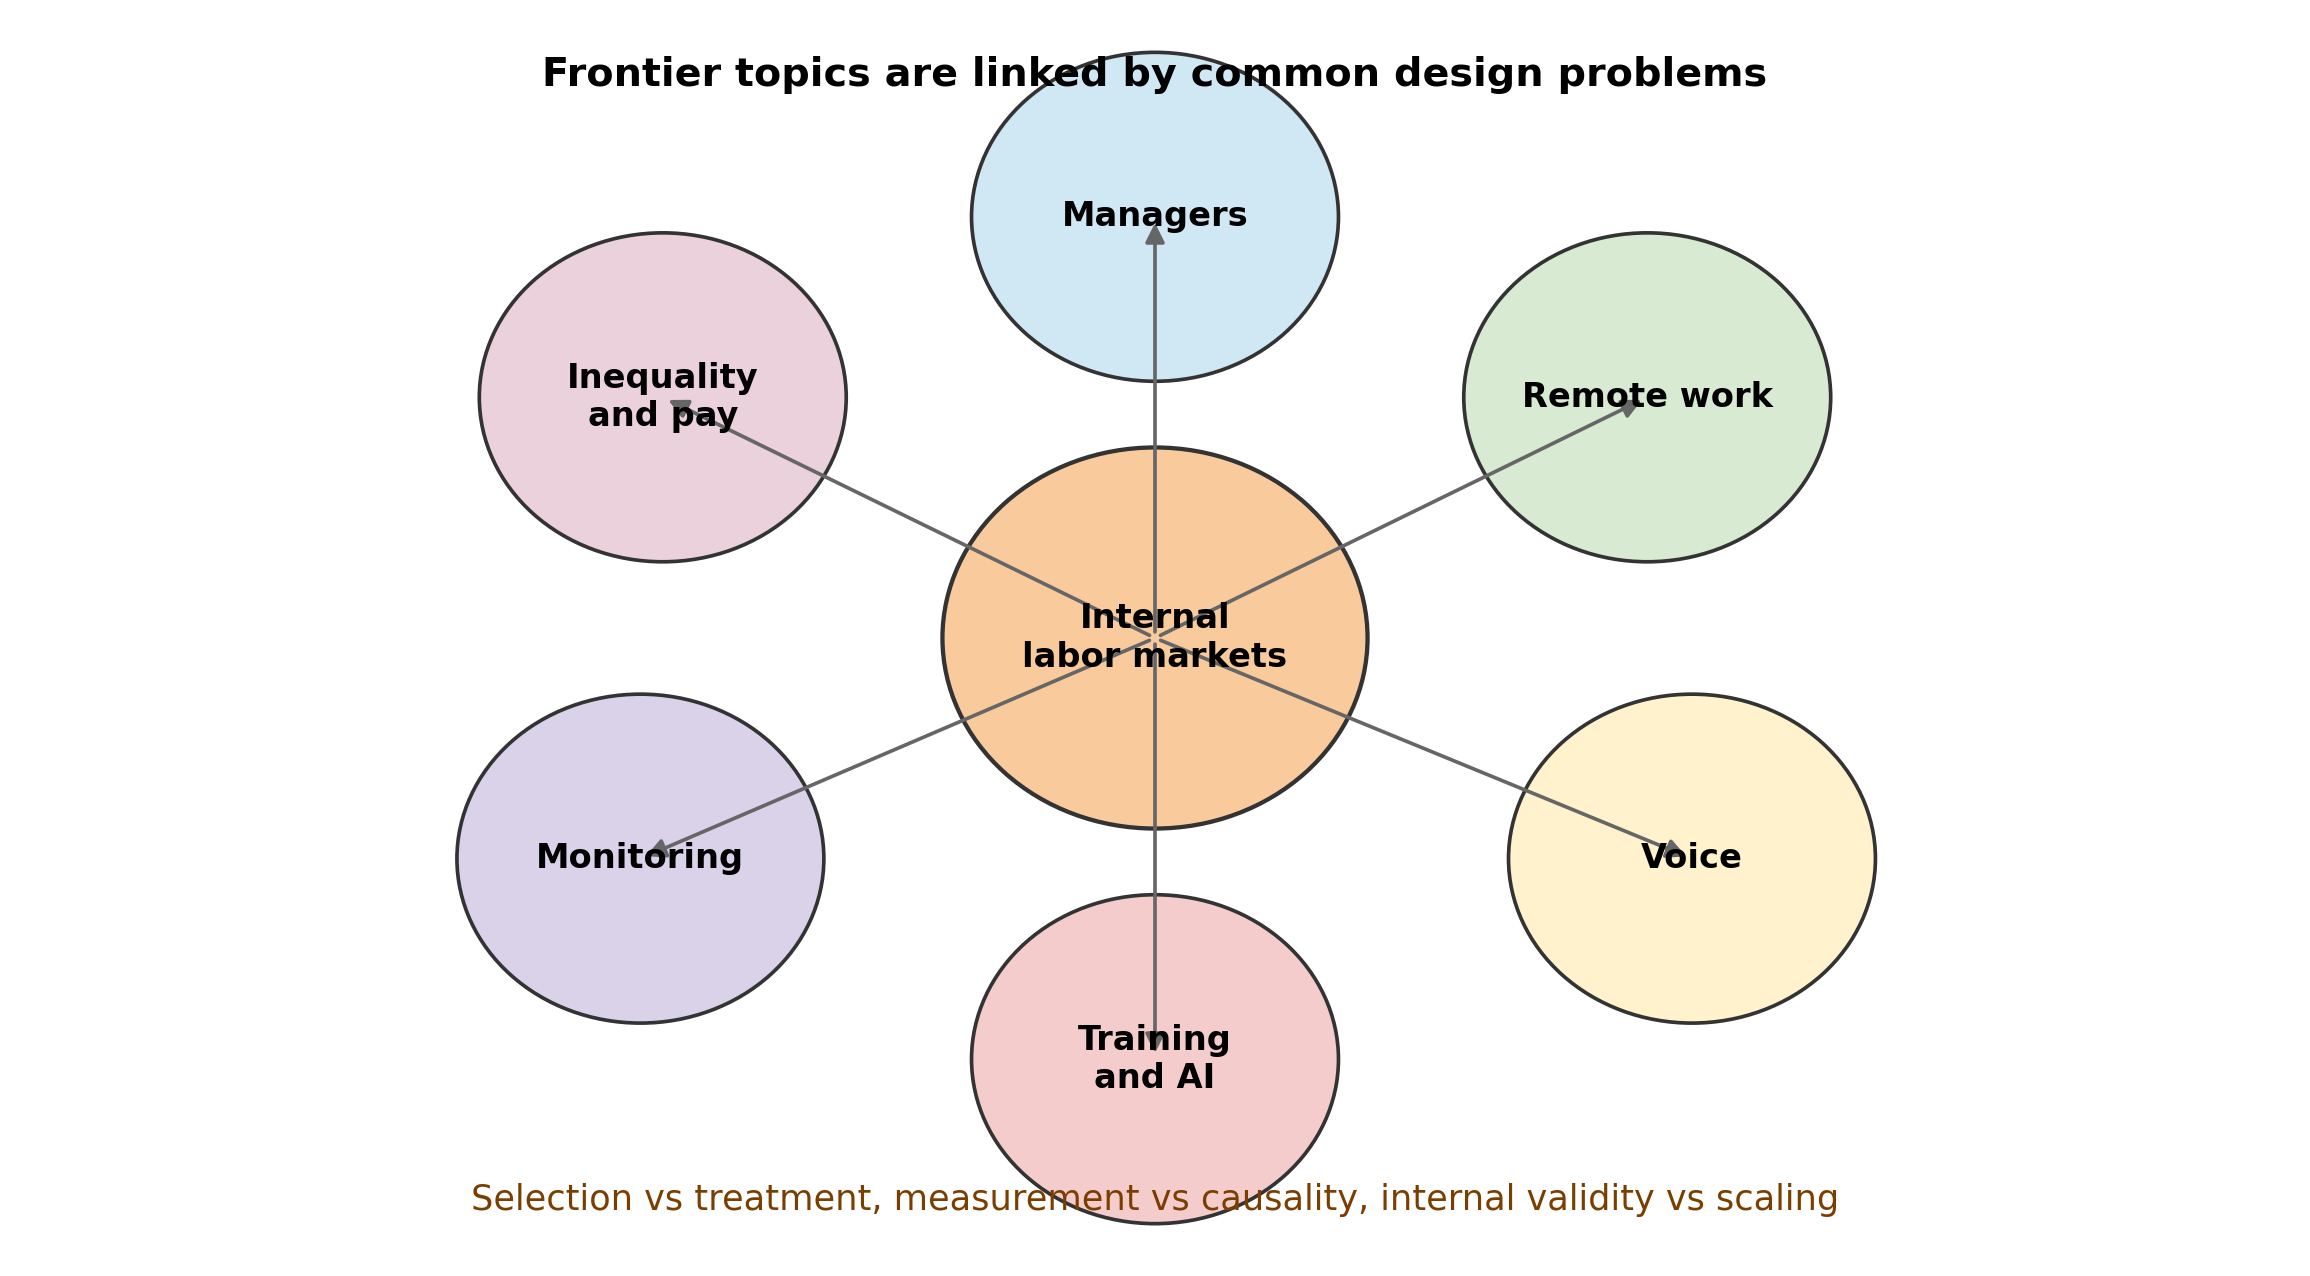
\includegraphics[height=0.68\textheight]{03-research-opportunities-landscape.png}
\end{center}
\end{frame}

\begin{frame}{Bridge to Week 4}
\begin{itemize}
    \item Personnel practices affect quits, internal hiring, retention, and vacancy filling.
    \item Week 4 takes these internal labor-market choices and studies worker flows across firms and unemployment states.
    \item Search and matching are easier to interpret once the inside of the firm is already clear.
\end{itemize}
\end{frame}

\begin{frame}{Takeaways}
\begin{itemize}
    \item Personnel economics studies incentives, evaluation, assignment, promotion, and organization inside firms.
    \item The key distinctions are effort versus sorting, assignment versus incentives, and managers versus peers.
    \item The best empirical habit is to name the variation, unit, observed margin, and external-validity caveat every time.
    \item Week 4 moves from internal labor markets to turnover, search, and unemployment flows.
\end{itemize}
\end{frame}

\end{document}
